\documentclass[10pt,conference,compsoc]{IEEEtran}
\usepackage{booktabs}
\usepackage{array}
\usepackage[hidelinks]{hyperref}
\usepackage{enumitem}
\usepackage{graphicx}
\usepackage{tikz}
\usetikzlibrary{arrows.meta,positioning}
\usepackage{xcolor}
\usepackage{balance}
\emergencystretch=2em

\setlist[itemize]{topsep=2pt,itemsep=1pt,leftmargin=1.3em}
\setlist[enumerate]{topsep=2pt,itemsep=1pt,leftmargin=1.5em}

\newcommand{\code}[1]{\texttt{\small #1}}
\newcommand{\sys}{MACE}
\makeatletter
\def\IEEEbibitemsep{0pt plus .5pt}
\makeatother

\title{MACE: A Multi-core Agentic Co-design Engine for Autonomous OpenPiton Bring-Up}
\author{\IEEEauthorblockN{Rana Umar Nadeem}
\IEEEauthorblockA{CHIA A3 Hackathon Submission, September 2026}}

\begin{document}
\bstctlcite{IEEEexample:BSTcontrol}

\maketitle

\begin{abstract}
MACE is an agentic AI system that builds and verifies multicore hardware on its own, running on
the CHIA framework. Phase 1 adds \code{chia\_openpiton}, a CHIA adapter exposing
OpenPiton's configure, build, simulate, run, and collect operations, validated with 208 tests. Phase
2 adds the MACE loop: a planner breaks a hardware objective into tasks, agents run them in parallel,
and a deterministic integrator gates every change against Verilator simulation before accepting it.
A failure-analysis agent diagnoses failures and the planner replans around them.

We tested MACE against two baselines, manual mesh scaling and a one-shot LLM prompt, on all three
supported cores, with every result taken from Verilator simulation of the RTL, not an agent's
self-report. We added PicoRV32 as a third core, resolving several RTL bugs that kept it from passing
under Verilator. We also found and fixed three OpenPiton bugs that kept 2x2 and 4x4 meshes from
passing; with them fixed, MACE's loop passes both sizes for Ariane and PicoRV32. The one-shot baseline failed on all three cores in three different ways; MACE
passed ariane and correctly stopped within its retry budget on the other two instead of reporting a
false pass. The artifact pins its toolchain in a Nix flake, entered with a single \code{nix develop}.
\end{abstract}

\begin{figure*}[t]
\centering
\vspace{-0.4em}
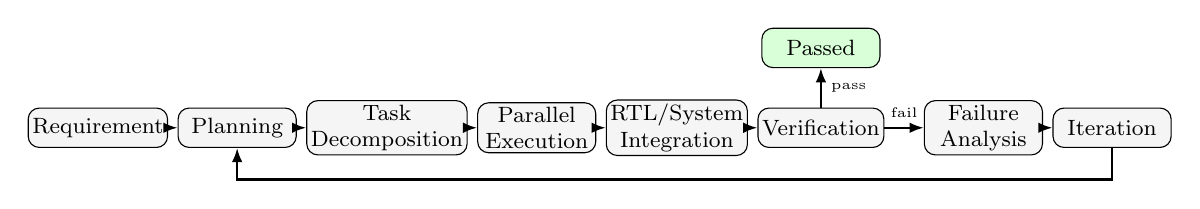
\begin{tikzpicture}[
    box/.style={draw, rounded corners, minimum height=0.5cm, minimum width=1.5cm,
                align=center, font=\footnotesize, fill=gray!8, inner sep=1.5pt},
    arr/.style={-{Latex[length=1.8mm]}, thick},
    lbl/.style={font=\tiny, midway}
  ]
  \node[box] (req) {Requirement};
  \node[box, right=0.12cm of req] (plan) {Planning};
  \node[box, right=0.12cm of plan] (dec) {Task\\Decomposition};
  \node[box, right=0.12cm of dec] (par) {Parallel\\Execution};
  \node[box, right=0.12cm of par] (int) {RTL/System\\Integration};
  \node[box, right=0.12cm of int] (ver) {Verification};
  \node[box, right=0.5cm of ver] (fail) {Failure\\Analysis};
  \node[box, right=0.12cm of fail] (iter) {Iteration};
  \node[box, above=0.5cm of ver, fill=green!15] (done) {Passed};
  \draw[arr] (req) -- (plan);
  \draw[arr] (plan) -- (dec);
  \draw[arr] (dec) -- (par);
  \draw[arr] (par) -- (int);
  \draw[arr] (int) -- (ver);
  \draw[arr] (ver) -- node[lbl, right]{pass} (done);
  \draw[arr] (ver) -- node[lbl, above]{fail} (fail);
  \draw[arr] (fail) -- (iter);
  \draw[arr] (iter.south) -- ++(0,-0.4cm) -| (plan.south);
\end{tikzpicture}
\vspace{-0.6em}
\caption{The MACE pipeline. Verification gates every integrated change against Verilator
simulation rather than an agent's self-report. The run ends when every gate workload passes; any
failure triggers failure analysis and a replan rather than a bare retry.}
\label{fig:pipeline}
\vspace{-0.4em}
\end{figure*}

\section{Introduction}

Current agentic coding systems are typically benchmarked on isolated tasks or toy
problems~\cite{humaneval,verilogeval}, which fails to capture the complexity of actual hardware
construction. Bringing up a multicore system means navigating a large RTL codebase
(OpenPiton~\cite{openpiton} spans hundreds of thousands of lines across
network-on-chip, cache-coherence, tile, and platform logic), a fragile toolchain (version skew,
cross-compilation bugs, checkout-specific issues), and verification that costs minutes to hours per
attempt rather than milliseconds.

MACE is designed for this high-friction environment. Given a hardware objective, such as ``bring up
a 2x2 mesh'' or ``verify workload $W$ passes,'' MACE plans, implements, builds, simulates, diagnoses
failures against Verilator~\cite{verilator} output, and iterates. Every claim of success is gated by Verilator
simulation; MACE never accepts an agent's self-report.

\subsection{Features}

MACE contributes:
\begin{itemize}
\item \code{chia\_openpiton} (Sec.~\ref{sec:phase1}): a CHIA adapter for OpenPiton with a full
configure/build/run/collect interface, built the same way as CHIA's gem5 and ESP adapters, so it can
be upstreamed directly.
\item The MACE loop (Sec.~\ref{sec:phase2}): planning, parallel task execution, deterministic
integration, and LLM-driven failure triage, tested end to end against full Verilator runs, with cost, time, and task
metrics.
\item A third core, PicoRV32 (Sec.~\ref{sec:pico}), brought up by fixing pre-existing bugs in its
upstream OpenPiton integration, which OpenPiton's continuous integration builds but never runs.
\item An interactive CLI and two further capabilities (Sec.~\ref{sec:cli}): Verilator code coverage as
a second verification axis, and a second working LLM backend.
\end{itemize}

\section{Background}

CHIA~\cite{chia} provides the agent, tool, and dispatch layer this project builds on: colocated
resource-pinned worker nodes, an LLM abstraction layer spanning multiple backends, and
Ray-based~\cite{ray} remote dispatch and caching. OpenPiton~\cite{openpiton} is Princeton's
open-source, silicon-proven manycore research framework. Tiles connect through a 2D-mesh
network-on-chip and speak a custom MESI-coherence protocol (L15, descended from OpenSPARC T1's
PCX/CPX bus) to reach the NoC. OpenPiton supports three tile cores, the latter two added through its
BYOC framework~\cite{byoc}: OpenSPARC T1 (\code{sparc}), Ariane/CVA6~\cite{cva6} (\code{ariane},
RV64GC, coherent), and PicoRV32~\cite{picorv32} (\code{pico}, RV32I, non-coherent). Before this
project, CHIA had no OpenPiton adapter.

\textbf{Related work.} LLM-based hardware design has mostly been evaluated at module scale.
VerilogEval~\cite{verilogeval} scores single-module Verilog generation, ChipNeMo~\cite{chipnemo}
adapts LLMs to chip-design tasks, and AutoChip~\cite{autochip}, RTLFixer~\cite{rtlfixer},
VerilogCoder~\cite{verilogcoder}, and MAGE~\cite{mage} feed compiler or simulation results back to
one or more agents to repair generated RTL. In software, SWE-bench~\cite{swebench} moved evaluation
from isolated functions~\cite{humaneval} to repository-level issues. \sys{} applies the same
agent-with-feedback idea at system scale: rather than writing one module against a small testbench,
it plans and verifies bring-up of an existing manycore, gated by whole-system Verilator simulation.

\section{Phase 1: The OpenPiton Adapter}
\label{sec:phase1}

\textbf{Design.} \code{OpenPitonWorkspaceNode} is a CHIA \code{ColocatedNode} exposing
\code{configure}, \code{build}, \code{run}, \code{regress}, \code{collect}, and \code{clean} as
resource-pinned remote functions. OpenPiton's template preprocessor writes generated \code{.tmp.v}
files into the source tree on every build, so the adapter gives each worker its own checkout,
reserved through one \code{openpiton} resource unit, instead of locking a shared one. Pure parsers
read build and run verdicts from OpenPiton's transcripts (\code{sim.log}, \code{status.log}), using
the strings its RTL monitors emit; a verdict never comes from an agent's claim.

\textbf{Environment hardening.} The build surfaced four infrastructure bugs, fixed in one
idempotent patch script: binutils~2.38+ splitting \code{zicsr}/\code{zifencei} out of base RV64I,
which breaks the boot ROM's assembly; GCC~15's C23 default breaking a legacy function call; broken
git symlinks on a Windows-mounted checkout; and CRLF shebangs in 66 files. A Nix
flake~\cite{nix} pins the toolchain, including a Verilator release (5.052) that avoids two Verilator
bugs this RTL triggers.

\textbf{Build-result caching.} \code{build()} skips the simulator when a matching successful-build
marker exists: rebuilding an identical configuration dropped from 104s to 0.00s, so an iteration
that only changes the test never rebuilds.

\textbf{Results.} 208 tests that need no OpenPiton checkout (pure-unit, and live-Ray with a stub
simulator) all pass. Acceptance tests with full Verilator builds pass for a 1x1 Ariane build and run
(\code{hello\_world.c}, compiled and executed by the adapter itself) and for two independent
checkouts building in parallel: 176s versus 324s serial. One acceptance test, 2x2 Ariane on a GCP
worker, remains blocked by upstream infrastructure dependencies (Sec.~\ref{sec:limits}).

\section{Phase 2: The \sys{} Loop}
\label{sec:phase2}

\textbf{Pipeline.} Figure~\ref{fig:pipeline} shows the loop. A planning agent turns a
\code{MaceSpec} (core, target mesh, gate workloads, objective, budget) into a task DAG, and workers
dispatch ready tasks in parallel through Ray, each pinned to its own checkout. A deterministic
integrator, with no LLM, applies accepted diffs in dependency order, then builds and runs every gate
workload; each workload's \emph{verdict}, parsed from simulator output, must read \code{pass}. On
any failure, a failure-analysis agent with read-only tools (log grep, file collection, a fixture
diff, and an \code{objdump} symbol check) diagnoses the transcript, and the planner replans around
its proposed fix.

\textbf{Gate workloads surface an RTL bug.} Writing the gate workloads (barrier-and-atomic-counter,
producer/consumer, hart-id scatter/gather) exposed a memory-visibility bug: a plain \code{volatile}
read of a shared value was not reliably visible from the same hart shortly after the write, while an
atomic fetch-and-add-zero read always was. Every gate workload now reads shared values through this
\code{atomic\_read()} helper.

\textbf{Resource enforcement.} \sys{} checks all three \code{Budget} dimensions (iterations, USD,
wall-clock) before each iteration starts, and verifies gate-workload checksums before any LLM call
or checkout access, so a task cannot tamper with its own grading. Every run in this paper together
cost \$37 of a \$300 GCP credit allocation, covering simulation compute and LLM inference;
development used a \$20/month Claude subscription, outside that budget.

\textbf{Deterministic replay.} \sys{} cache-tags LLM, build, and run decisions and re-serves them at
no token or compute cost. Per CHIA's cache implementation, this replays \emph{decisions} (response
text, pass/fail artifacts), not the source edits an agent made; those remain git's job.

\section{A Third Core: PicoRV32}
\label{sec:pico}

Integrating arbitrary core RTL into OpenPiton means navigating fundamental architectural
differences rather than wiring up a standard bus. OpenPiton has no reusable core-to-NoC bridge:
under BYOC, each core reaches the L15 through its own transducer, and even Ariane's AXI4 output goes
unused, since a hand-written encoder taps CVA6's internal pre-AXI cache-miss stream instead. The
dividing line is whether the core has its own coherent cache, not whether it speaks a standard bus:
a new core with one, as Ariane has, needs new coherence-adapter RTL, beyond this project's timeline.
PicoRV32 does not: a complete, TODO-free upstream transducer (\code{pico\_l15\_transducer.v} and
friends) already exists. OpenPiton's CI builds it under Verilator but never runs it: the run job is
commented out, targets a nonexistent stage, and even when live pointed at a different simulator.

\textbf{Results.} The adapter extension (a new \code{Literal} entry, two \code{sims} flags, mirrored
tests) landed with full unit coverage and no regressions to the \code{ariane} and \code{sparc}
paths. The build takes 57 seconds, faster than Ariane's since it skips the bootrom/device-tree
chain, but the first run ended at \code{maxcycles}. The binary's symbols and entry point matched the
run's trap addresses (\code{objdump~-t}/\code{-f} against \code{symbol.tbl}), ruling out a build or
toolchain mismatch, and its transcript matched a passing Ariane fixture line for line until the
fixture's \code{Hit Good trap}, which never appeared: the core itself never reached its trap address.

Waveform tracing found three RTL/testbench bugs: PicoRV32's \code{resetn}/\code{booted}
self-boot gate, the manycore monitor's \code{active\_thread} tracking for pico's tile, and the SRAM
model's power-on BIST self-clear, which discarded pico's first memory writes. With all three fixed, PicoRV32 \textbf{passes} under Verilator (\code{Simulation -> PASS (HIT GOOD
TRAP)}). The bugs surfaced only because \sys{} separates a successful build from a correct run
instead of reporting a false pass.

\textbf{Multi-tile pico.} The fixes generalize: on 2x2 and 4x4 meshes, every tile reaches
\code{Hit Good trap} on \code{addi.S} (\code{Simulation -> PASS}). \code{barrier\_atomic.c} never
runs on pico at any mesh size, for a simpler reason: pico's OpenPiton integration has only an
assembler, no C compiler or \code{crt.S}/\code{syscalls.c}, so the diag never compiles and every tile
idles at its reset vector on an empty memory image. This is a toolchain gap, not an RTL bug, and not
the workload/mesh mismatch an earlier, unverified triage diagnosis assumed. The atomic hardware that
workload needs does work: the upstream \code{amoadd\_w.S} test, pure assembly, passes on pico.

\section{Additional Capabilities}
\label{sec:cli}

\sys{} features a standard EDA-style interactive shell (modeled on Yosys/OpenROAD) that validates
core compatibility up front to prevent invalid integration attempts. To provide a second verification
axis beyond pass/fail, we patched the OpenPiton testbench to call Verilator's coverage-write API,
yielding metrics such as 36.00\% line coverage for a 1x1 Ariane run. The agentic loop is also
backend-agnostic, running unmodified against Google Vertex Gemini and OpenCode, each confirmed with a
full passing run.

\section{Evaluation}
\label{sec:eval}

We compare three approaches: \textbf{(a)} manual mesh scaling with a time log, \textbf{(b)} a single
LLM prompt for a configuration applied once with no tools, verification, or retry, and \textbf{(c)}
the full \sys{} loop.

\textbf{Three cores, two baselines.} We ran (b) and (c) on the same objective, verify
\code{barrier\_atomic.c} on a 1x1 mesh, for all three cores, with Gemini~2.5~Flash throughout
(Figure~\ref{fig:eval}, left).

\begin{figure*}[t]
\centering
\vspace{-0.8em}
\begin{minipage}{0.5\textwidth}
\centering
\footnotesize
\begin{tabular}{@{}lll@{}}
\toprule
\textbf{Core} & \textbf{(b) one-shot LLM} & \textbf{(c) full loop} \\
\midrule
ariane & {\color{red!60!black}fail}, 186.5s & \textbf{\color{green!50!black}pass}, 741.7s \\
sparc & {\color{red!60!black}fail}, 766.0s & {\color{orange!80!black}budget\_exceeded}, 966.3s \\
pico & {\color{red!60!black}fail} (unparseable), 32.6s & {\color{orange!80!black}budget\_exceeded}, 1250.5s \\
\bottomrule
\end{tabular}
\end{minipage}%
\hfill
\begin{minipage}{0.46\textwidth}
\centering
\footnotesize\textbf{ariane}, \code{barrier\_atomic.c}\\[2pt]
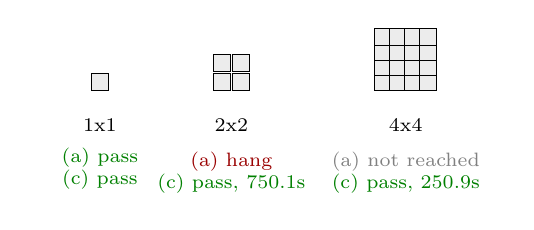
\begin{tikzpicture}[tile/.style={draw, fill=gray!15, minimum size=0.22cm, inner sep=0}, font=\scriptsize]
  \node[tile] at (0,0.55) {};
  \node at (0,0.0) {1x1};
  \node[align=center, text width=1.6cm] at (0,-0.55)
    {{\color{green!50!black}(a) pass}\\{\color{green!50!black}(c) pass}};

  \foreach \x in {0,1} \foreach \y in {0,1} \node[tile] at (1.55+\x*0.24,0.55+\y*0.24) {};
  \node at (1.67,0.0) {2x2};
  \node[align=center, text width=2.3cm] at (1.67,-0.6)
    {{\color{red!60!black}(a) hang}\\{\color{green!50!black}(c) pass, 750.1s}};

  \foreach \x in {0,...,3} \foreach \y in {0,...,3} \node[tile] at (3.6+\x*0.19,0.55+\y*0.19) {};
  \node at (3.885,0.0) {4x4};
  \node[align=center, text width=2.3cm] at (3.885,-0.6)
    {{\color{gray}(a) not reached}\\{\color{green!50!black}(c) pass, 250.9s}};
\end{tikzpicture}
\end{minipage}
\vspace{-0.4em}
\caption{\textbf{Left:} all three cores, same 1x1 objective. (b) never passes. On sparc/pico, (c)
exhausts its retry budget instead of reporting a false pass; only ariane
\textbf{\color{green!50!black}passes}, under (c). \textbf{Right:} manual mesh scaling (a) vs.\ (c),
ariane only.
{\color{green!50!black}Green}=pass, {\color{red!60!black}red}=hang, {\color{gray}gray}=not reached.
The loop passes both shapes (a) got stuck on.}
\label{fig:eval}
\vspace{-0.4em}
\end{figure*}

(b) fails all three cores, each in a different way. On ariane, the one-shot config built but failed
verification: a wrong guess. On sparc, it built and reached a run attempt that failed silently, with
no verdict at all. On pico, \code{PitonConfig}'s construction-time validation rejected the LLM's
config (\code{l15\_size=0}) before any simulation ran; (b) has no retry path for a malformed response.

(c) passes ariane: 4/4 tasks, 741.7s, about 4x (b)'s cost. A second ariane gate workload,
\code{producer\_consumer.c}, also passed (2118.02s, 2 tasks), coverage beyond one program. On sparc
and pico, (c) exhausts its retry budget on \code{barrier\_atomic.c} instead of passing; \sys{}'s
triage and post-mortem told the two failures apart, and we verified both independently.

sparc's failure has two layers. The first is an ISA gap: \code{barrier\_atomic.c} uses
\code{util.h}'s \code{ATOMIC\_FETCH\_OP} macro, which is RISC-V inline assembly, and OpenSPARC T1
has no C diag environment, so no portable fix exists. Pure-assembly diagnostics, including
OpenPiton's CI-verified \code{princeton-test-test.s}, avoid that gap but expose a second: every sparc
run reached \code{max\_cycle} with no verdict, because \code{pc\_cmp.v.pyv}'s \code{RTL\_SPARC0}
branch never assigned \code{active\_thread}, unlike the Ariane and pico branches. Mirroring their
pattern fixed the monitor, which now tracks all four threads and reports \code{FAIL(TIMEOUT)}
instead of silence. The threads themselves still make no forward progress, even at 100x the default
timeout; that remains open.

\sys{}'s triage blamed pico's failure on a workload/mesh mismatch (a 1x1 mesh cannot supply
\code{barrier\_atomic.c}'s multi-participant barrier). That unverified LLM diagnosis was wrong:
\code{barrier\_atomic.c} never compiles for pico at any mesh size (Section~\ref{sec:pico}). On
\code{addi.S}, the loop passes pico in one task at every size, end to end: 1x1 in 115.5s, 2x2 in
70.7s, and 4x4 in 293.2s. That needed one new
capability, a \code{CONFIG\_RTL:} planner directive so a task can request
\code{CONFIG\_DISABLE\_BIST\_CLEAR} on top of the mesh's defaults. The fix was named in the
objective, so this shows the loop applying a known fix, not discovering one.

\textbf{The loop passes mesh shapes where manual scaling stalled.} Baseline (a), run before any
fixes, stalled at 2x2 and never reached 4x4, due to latent upstream bugs, chiefly a stale-read exit
barrier in \code{syscalls.c} and a 32-bit \code{finish\_mask} that capped verification at 8 tiles.
After we patched them by hand, the loop planned and verified both meshes, every tile confirmed, with
no changes to its planning or verification logic (Figure~\ref{fig:eval}, right): 2x2 in 750.1s
across four tasks, including an L1D-associativity variant the planner chose to verify, and 4x4 in
250.9s on a cached build.

Phase~2's fan-out (two tasks, two checkouts, through baseline (c)'s path) measured 30s parallel
versus 57s serial, matching Phase~1's result.

One validation limitation remains: the detect-failure, diagnose, replan, pass cycle is proven only
at the mechanism level (a stateful stub that fails once, then passes). No passing run above needed
it, not even a forced extreme first config (a 128-byte, direct-mapped L1, confirmed in the build)
that we and the planner both expected to fail. The one real failure it met, a pico 4x4 build cached
before the \code{finish\_mask} fix, it did not recover from: a build ID covers configuration, not
source edits, so all three replans reused the stale build while triage blamed the RTL. A clean
rebuild passed.

\section{Limitations and Open Issues}
\label{sec:limits}

\textbf{GCP dispatch.} A task needing a tailnet-relayed GCP worker first never ran because CHIA sets
three proxy environment variables during \code{chia up} that \code{chia job submit} inherits but
our manually launched drivers did not; exporting them took the task from a six-minute hang to a
two-second run. A later attempt on the same topology hung again with that fix in place, and relay
logs plus a raylet \code{strace} show no outbound activity, pointing at Ray's scheduling under a
proxied topology rather than CHIA. That follow-up remains open.

\textbf{Future work: generality over one-off adapters.} All three cores here already had upstream
OpenPiton/L15 adapters (SPARC's CCX transducer, Ariane's L15 adapter in CVA6, PicoRV32's
transducer); a core without one, such as Ibex or Rocket Chip, needs it written first. The existing
three share a shape: a per-core RTL directory, a transducer between the core's memory interface and
L15, and a core-select arm in the tile template. The next step is turning that shape into a template
and adding 2-4 more cores, with \sys{}'s loop verifying each iteration of the adapter RTL in
Verilator while a hardware engineer writes it. A second direction is a dashboard over the run
database, showing dispatch, build, and verification live instead of through raw trace files.

\balance
\section{Conclusion}

\sys{} shows that an agentic loop can plan, build, and verify multicore hardware, gated by RTL
simulation instead of an agent's word. Along the way we fixed environment and RTL bugs and added a
third core, and the loop then passed 2x2 and 4x4 meshes of both Ariane and PicoRV32.
Precision, not a single pass, is the point.

\bibliographystyle{IEEEtran}
\bibliography{mace_paper}

\end{document}
